
\documentclass[aspectratio=169]{beamer}
\usepackage[utf8]{inputenc}
\usepackage[T1]{fontenc}
%%%%%%%
% \usepackage{layout}
% \usepackage{lipsum}
%%%%%%%
\usetheme[% Complete settings. Default value in []
% titleimagecolor=red,       % [gray], darkgray, red, blue, green
% titleimagemargin=2mm,      % Distance [2mm]    Frame around title page image
% navigationsymbols=false,   % true   / [false]  Navigation symbols in the foot
% mathseriffont=false,       % true   / [false]  Serif / non-serif math fonts
% foot=true,                 % [true] / false    Footline or not
% nofootslidenum=false       % true   / [false]  Keep slide num even when foot=false
% footlogo=true,             % [true] / false    Put LU logo to the left of footer
% english=true,              % [true] / false    English / Swedish logo
% LTHlogo=false,             % true   / [false]  Use LTH logo instead of LU on title and end pages.
% blackenumeratenumber=true, % [true] / false    Black enumerate numbers, o.w. Lund bronze
% blackitemmark=false,       % true   / [false]  Black item marks, o.w. Lund bronze
% defaultfont=false,         % true   / [false]  Falls back to default beamer fonts
% sectionframe=true,
]{ulund}
%%%%%%%%%%%%%%%%%%%%% Layout commands 
%%%% Foot
% \ulundfootleft{\insertshortauthor}
% \ulundfootmid{\insertshorttitle}
% \ulundfootright{\insertframenumber}% {\insertframenumber:\inserttotalframenumber}
%%%% Titleimage
\titleimage{Pictures/ULUNDcolor} % Replaces the LU image. Voids option titleimagecolor
%%%%%%%%%%%%%%%%%%%%%%%%%%%%%%%%%%%
\title[LUFOSS]{LUFOSS: \vspace{0.25em}\newline \fontsize{16}{25}\selectfont Lund University Fund for\\Open Source Software }
\author[www.lufoss.org]{%
  Chair: Prof. Björn Regnell\newline
  Dept.\@ of Computer Science, Lund University}
%%%%%%%%%%%%%%%%%%%%%
\usepackage{verbatim}
%%%%%%%%%%%%% Verbatim code box
\usepackage[skins,listings]{tcolorbox}
\tcbuselibrary{listingsutf8}

\usepackage{pgf-pie}

\newcommand{\TitleSlide}{\begin{frame}[plain]\titlepage\end{frame}}

\newcommand{\EndSlide}{\begin{frame}[plain]\endpage\end{frame}}


\newcommand{\Section}[1]{\titleimagecolor{red}\section{#1}}

\newcommand{\code}{\lstinline[basicstyle=\ttfamily]}

\newenvironment{Slide}[1]%
  {\begin{frame}[environment=Slide]{#1}}
  {\end{frame}}%

% \newenvironment{Slide}[2][]  /// AAARGH strange error???
%   {\begin{frame}[fragile,environment=Slide,#1]{#2}}
%   {\end{frame}}



\begin{document}

\TitleSlide

%%%%%%%%%%%%%%%

\begin{Slide}{What is LUFOSS?}
\begin{itemize}
    \item Lund University Fund for Open Source Software
    \item \url{http://www.lufoss.org}
    \item \textbf{Mission}:
    \item[] Open Source Software (OSS) is not only changing our society, but a great way to learn about software development and to get a track record as a junior developer. LUFOSS gives scholarships to persons that contribute to OSS projects with significant utility and impact. Nominees can be students, doctoral candidates, and software developers in their early careers.
\end{itemize}
\end{Slide}

\begin{Slide}{What are the objectives of LUFOSS?}
  Lund University Fund for Open Source Software wants to ...
      \begin{itemize}
        \item encourage OSS activities among students, doctoral candidates, and young software developers in their early careers
        \item  encourage the industry in the Öresund region to use and contribute to OSS
        \item  initiate exchange between students working with OSS and the Öresund software industry
    \end{itemize}
    The LUFOSS nomination commitee decides about scholarships and prizes based on proposals that are assessed in relation to the criteria below. Anyone can propose candidates at \url{http://www.lufoss.org}  
  \end{Slide}
  


\Section{The LUFOSS Prize 2019}

\begin{Slide}{This years focus: OSS in teaching}
\begin{minipage}{0.5\textwidth}
  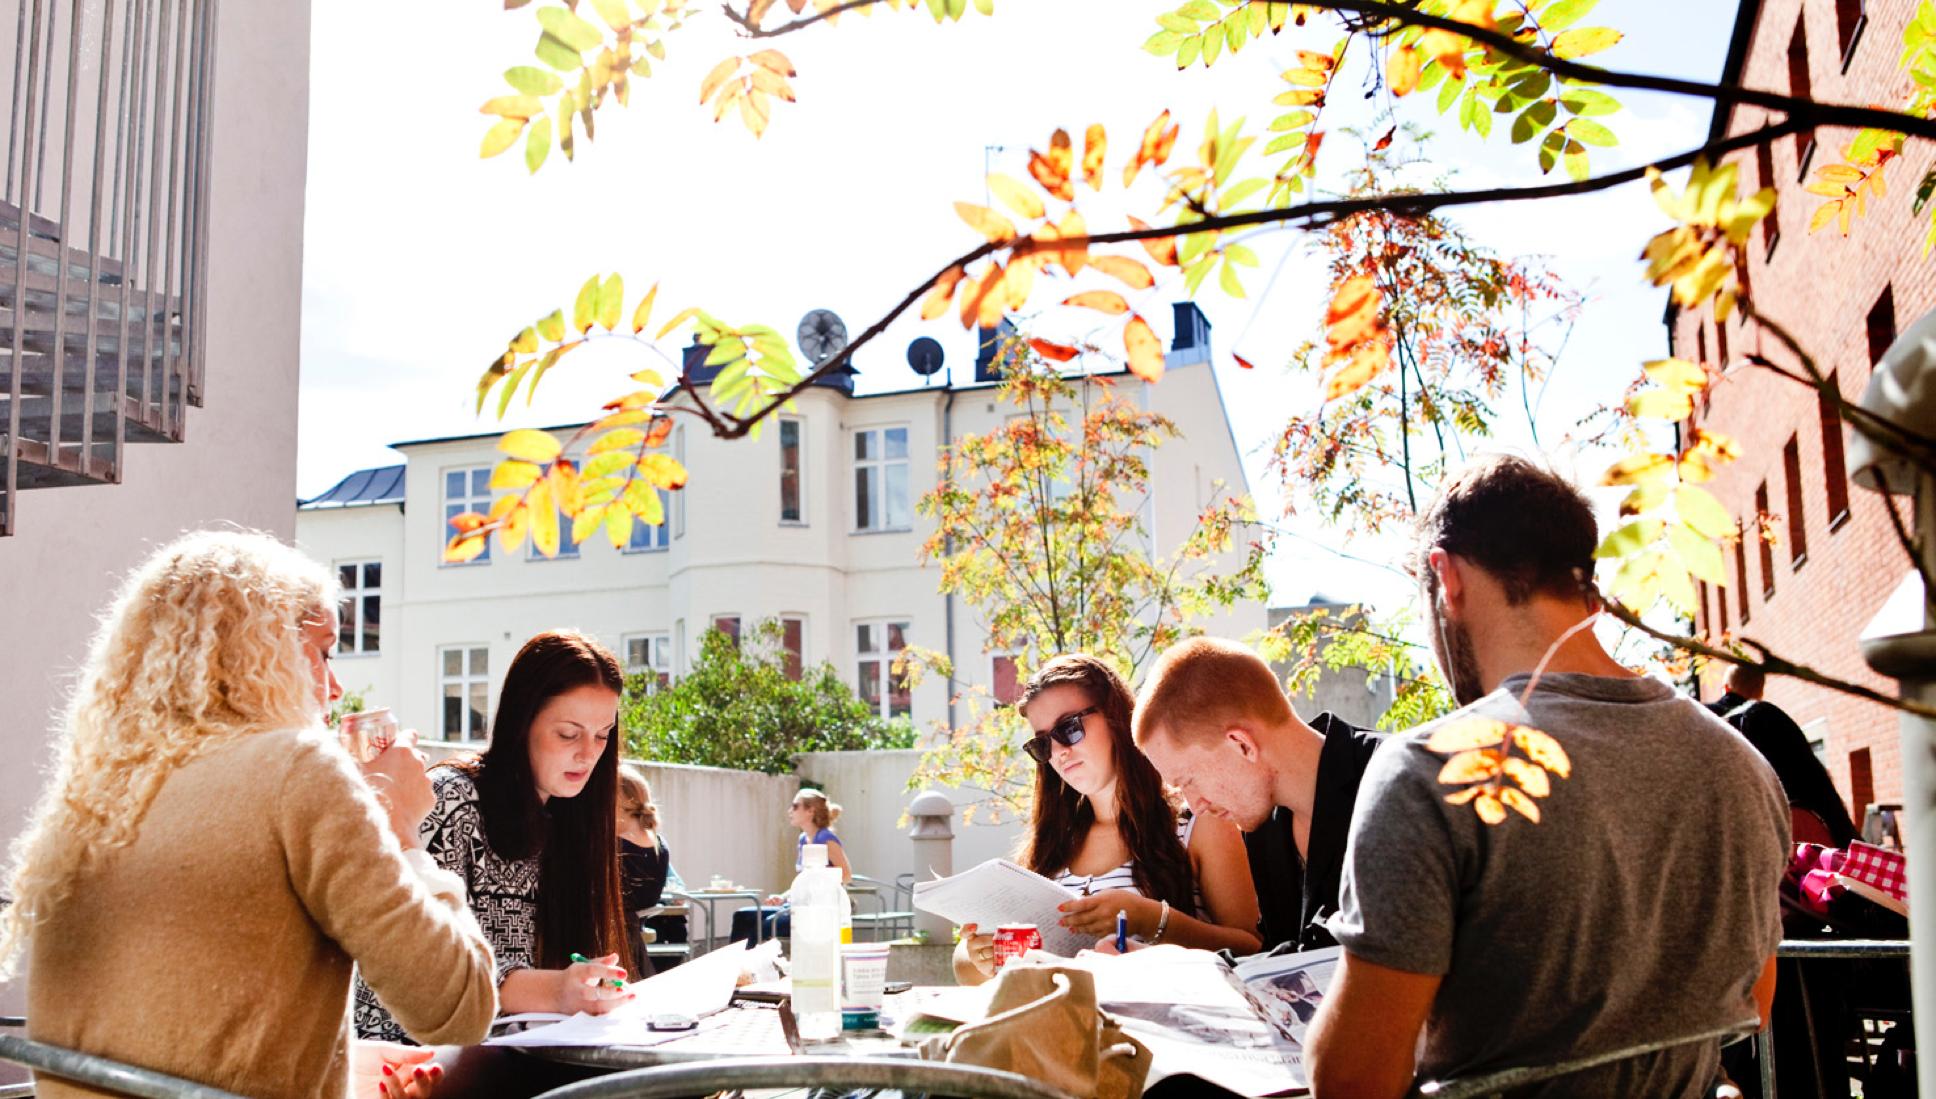
\includegraphics[width=1.0\textwidth]{Pictures/titlepictureGroup}
\end{minipage}%
\begin{minipage}{0.5\textwidth}
  \begin{itemize}
    \item Learning as an OSS project effort
    \item Students collaborate while learning using software repositories and git
    \item Teaching material as OSS with students as contributors
  \end{itemize}
\end{minipage}

  \end{Slide}

\begin{Slide}{The 2019 LUFOSS Prize winners are...}
~\pause
\begin{itemize}
  \item Sara Gunnarsson
  \item Peter Larsson
  \item Sara Månsson
  \item Erik Mårtensson
  \item Jonathan Sönnerup
\end{itemize} 
~\\~\\Pristagarna får dela på \pause\textbf{10 tusen kronor}!
\end{Slide}

\begin{Slide}{Prismotivering för LUFOSS-priset 2019}
    Sara Gunnarsson, Peter Larsson, Sara Månsson, Erik Mårtensson och Jonathan Sönnerup har som doktorander vid LTH arbetat aktivt med att främja öppen källkod som ett pedagogiskt verktyg.
    De har bland annat gjort en intressant undersökning av hur studenters engagemang kan ökas genom öppen källkod och kollektivt ägande av kursmaterial. 
    Arbetet är förmedlat till en bredare publik genom en läsvärd artikel publicerad vid LTH:s pedagogiska inspirationskonferens, som laddats ner flitigt och även citerats i Proceedings of the 50th ACM Technical Symposium on Computer Science Education. 
 

  {~\\\footnotesize\url{https://portal.research.lu.se/ws/files/27854342/group1_github_final.pdf}}

  {\footnotesize\url{https://dl.acm.org/citation.cfm?id=3287460}}
 
  \end{Slide}

  \begin{Slide}{Prize motivation for the 2019 LUFOSS prize}
    Sara Gunnarsson, Peter Larsson, Sara Månsson, Erik Mårtensson and Jonathan Sönnerup have as PhD students at Lund University worked actively to promote open source as a pedagogical tool. Their work include an interesting study of how students' engagement can be increased through open source software and collective ownership of teaching material. They have brought their work to a broader audience through a well-written paper presented at a pedagogical development conference. The paper has many downloads and has been cited in an artikel in the Proceedings of the 50th ACM Technical Symposium on Computer Science Education. 
 

  {~\\\footnotesize\url{https://portal.research.lu.se/ws/files/27854342/group1_github_final.pdf}}

  {\footnotesize\url{https://dl.acm.org/citation.cfm?id=3287460}}
 
  \end{Slide}


\end{document}